% !TEX root = thesis.tex
\chapter{深層学習のアルゴリズム}
Deep Learningは、多層ニューラルネットワークのアイデアをさらに一歩推し進めたもので、学習方法の工夫により、従来よりも多くのレイヤーを扱えて、より複雑な関数を学習できるようになった。数々の分類タスクにて、従来手法を大きくしのぐ成果を収め、注目を浴びている。この章では、Deep Learningがこれまで挙げた成果を紹介すると共に、Deep Learningで使われているアルゴリズムの詳細について述べる。

\section{深層学習の歴史}
多層ニューラルネットワークの学習方法は長らく困難とされてきたが、2006年にHintonらによって、多層のRBMを学習させる方法が発見され、発展への道が開けた\cite{hinton2006a-fast}。この研究では、RBMの重みを入力側から1層ずつ順に教師無し学習させ、学習済みの層は固定してしまうことにより、最終的に3つの隠れ層をもつニューラルネットワークによるモデルを学習させ、画像認識のタスクにて良い性能を発揮させることが出来るようになった。このRBMが複数層重なったモデルは、Deep Belief Network(DBN)と呼ばれた。\par
2012年には、1章でも述べたように、GoogleがYoutubeビデオの静止画を使って多層ニューラルネットワークの教師なし学習を行わせ、結果として、猫を認識するユニットや人を認識するユニットを学習させることに成功した。\par
%Deep Learningの登場 Hinton, Bengio, LeCun
%画像認識タスクでの成績、音声認識タスクでの成果、猫認識
%MNIST, CIFAR, SVHNなどにおけるconv.net、Maxout, DropConnectの優位

\section{深層学習モデルのバリエーションと詳細}
この節では、Deep Learningのアルゴリズムが、どのような要素の組み合わせで出来ているのか、それぞれの要素はどのようにして学習を助けているのか、紹介する。
%\subsection{pretraningとfinetuning}
\subsection{ネットワーク構造}
(MLP, SDA, DBM, CNN)
\subsection{Dropoutとrobustnessの確保}
Dropoutとは、2012年にHinton氏らによって提案された、過学習を防ぐための技術である\cite{hinton2012improving}。過学習とは、機械学習全般において、学習モデルが訓練で見たデータへの適応を重視し過ぎたために、未知のデータをうまく識別できなくなる現象のことを指す。Dropoutでは、過学習を防ぐため、各レイヤーからの出力をランダムに消去してしまう。これにより、各ユニットが他のユニットに頼らず自力で学習をする必要が生じ、より堅固(robust)な表現が獲得される、と考えられている。\par
DropConnectは、Dropoutをさらに一般化した手法である。DropConnectでは、各ユニットからの出力ではなく、ユニット同士のつながりをランダムにカットしている。
図\ref{c3_dropconnect}は、DropConnectの著者による紹介Webページ\footnote{\url{http://cs.nyu.edu/~wanli/dropc/}}に掲載されている画像の引用である。ニューラルネットワークにおけるニューロン同士の接続が、ランダムに切断されている様子を表している。
\begin{figure}[tbp]
 \begin{center}
  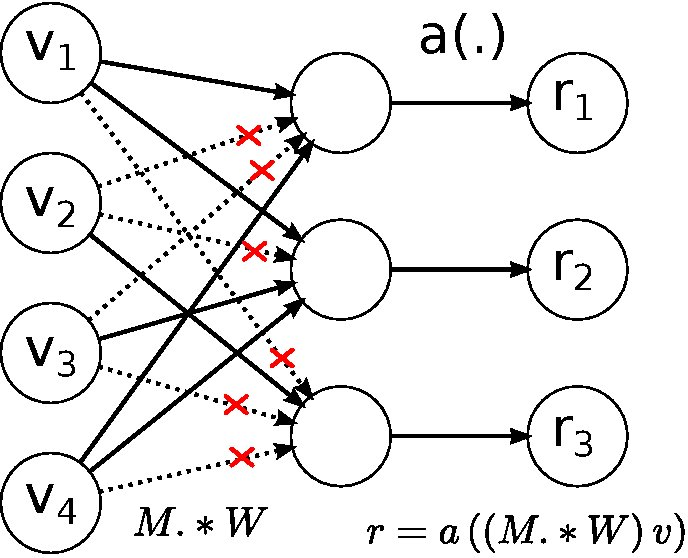
\includegraphics[width=50mm]{img/c3/nn_dc}
 \end{center}
 \caption{DropConnectの模式図}
 \label{c3_dropconnect}
\end{figure}
\subsection{活性化関数}
各ユニットに入力された値は、ある一定の関数によって増幅・変換される。これは人間の神経細胞を真似た仕組みで、神経細胞の化学物質による活性化にちなんで、活性化関数(activation function)と呼ばれる。この項では、Deep Neural Netを構成するときによく用いられる活性化関数を紹介する。
\subsubsection{sigmoidとhyperbolic tangent}
\subsubsection{rectifier}
\subsubsection{Maxout Unit}
Maxout Networkとは、バックプロパゲーションを伴う単純な多層MLP構造に、Dropout法を組み合わせ、さらにMaxout Unitという特殊な活性化関数を併用したニューラルネットワークである。\par
Maxout Unitでは、線形ユニットの出力を複数まとめて、それらのmaxを取る。さらに、複数のmaxout unitの線形和を取ることで、任意の連続関数を近似出来る。\par
図\ref{c3_maxout_app}は、maxout unitが複数の線形ユニットのmaxを取ることによって、様々な凸関数を近似出来る様子を、1次元の入力について示している。
\begin{figure}[tbp]
 \begin{center}
  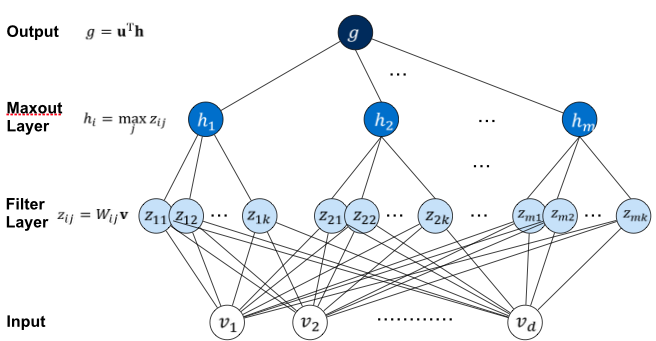
\includegraphics[width=100mm]{img/c3/maxout_arch}
 \end{center}
 \caption{Maxout Networkの構造図}
 \label{c3_maxout_arch}
\end{figure}
\begin{figure}[tbp]
 \begin{center}
  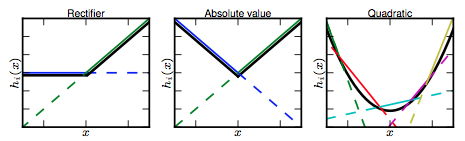
\includegraphics[width=100mm]{img/c3/maxout_app}
 \end{center}
 \caption{Maxout Unitが凸関数を近似する様子(1次元の場合)}
 \label{c3_maxout_app}
\end{figure}
